\documentclass[12pt]{extarticle}
\usepackage[english]{babel}
\usepackage[utf8]{inputenc}
\usepackage{amsmath}
\usepackage{graphicx}
\usepackage[colorinlistoftodos]{todonotes}
\usepackage[hidelinks]{hyperref}
\usepackage{courier}
\usepackage{booktabs}
\usepackage[T1]{fontenc}
\usepackage{tabularx}
\usepackage[margin=0.5in]{geometry}

\begin{document}
\begin{center}
\bf \Huge BoxIn\\
Developer Guide

\includegraphics[width=\textwidth]{BoxIn}
\end{center}

\pagebreak

\tableofcontents

\pagebreak

\section{Background}

BoxIn is a C++ based to-do list manager and this guide will help to understand how it works. BoxIn design adheres to the following coding standards

\subparagraph{SLAP}    
SLAP refers to Single Level Abstraction Principle. Code should be well abstracted so that each function only has one level of function calls. This helps to keep code from becoming convoluted by abstracting away the details of how a function is implemented

\subparagraph{Memory Management}
Coding in C++ requires efficient use of memory. Memory should be freed if its not in use any longer.

\subparagraph{Compatibility}
Code should be written such that is is cross platform and compatible with different compilers. Compiler specific code should be marked as such.

\subparagraph{Coding standard}
BoxIn code follows the coding standard listed out here: \href{https://docs.google.com/document/pub?id=1tJD2XQo3hUb0SZniswLqg0vkmccv7vGBV7\_1AhTYK04\&amp\&embedded=true}{C++ coding standards}.

\subparagraph{Namespaces}
All namespaces should be marked out to avoid confusion with the Boost library which is used in many parts of the code. For example, \texttt{std::string} rather than simply \texttt{string}

\newpage

\section{Anatomy}

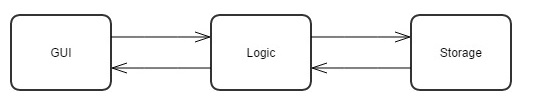
\includegraphics[width=\textwidth]{architecture}

BoxIn has 3 major components, the GUI, the Logic and the Storage components. The components are divided in a way that follows two guiding principles. We also apply the Model View Controller pattern. A full class diagram is available in the Appendix

\subsection{Model View Controller pattern}
In BoxIn, the GUI component acts as both the View and the Controller. Users view all events through the GUI and the GUI is also responsible for taking care of all user interaction, including mouse clicks and information sent through the command line. More details are found in Section 3.
The Model in the system is the Event class. More details are found in Section 5.

\subsection{Separation of Concerns}
Each major component of the application handles it's own concerns. For example, the GUI or Storage components do not process any command line input, only the Logic does.

\subsection{Law of Demeter}
This law is particularly effected in the fact that the GUI and the Storage classes have no knowledge of each other - neither calls any functions of the other.


\newpage
\section{GUI}

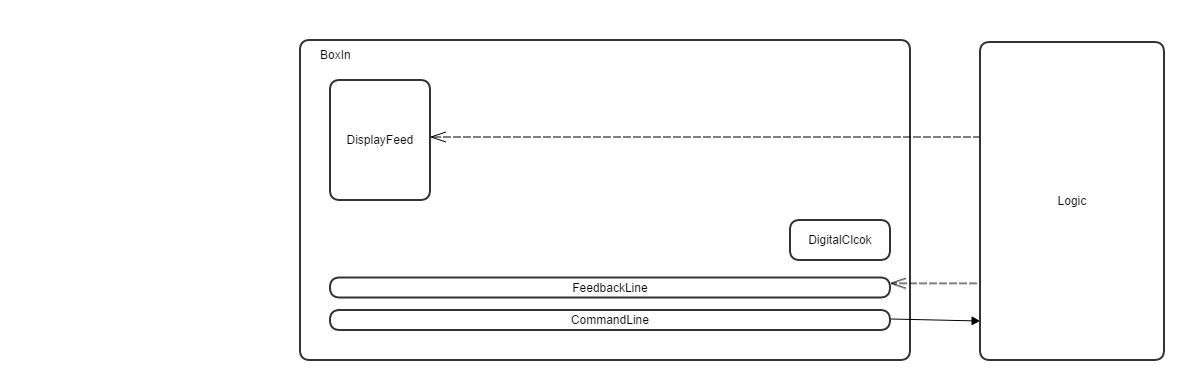
\includegraphics[width=\textwidth]{component_design_gui}
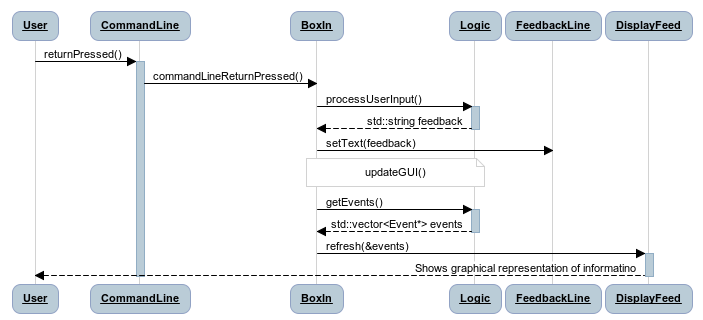
\includegraphics[width=\textwidth]{gui_sequence_diagram}
The GUI component acts as both the controller and the view in the MVC pattern. The library used to is the Qt library. The documentation for the Qt library is available here: \href{http://qt-project.org/doc/}{http://qt-project.org/doc/}\\
The above diagrams give a graphical representation of how the \texttt{GUI} is designed in both the sequential calls on user actions and as a component.
The GUI is divided into 5 components, discussed below

\subsection{BoxIn (main window)}
The \texttt{BoxIn} class is the main window. The majority of setup for this window is done in a \texttt{.ui} file generated using Qt Creator. All other sub-components found in this window should also have this window as a parent window. This class inherits from \texttt{QWidget}. The \texttt{BoxIn} class mainly acts as a container for all other classes for presentation's sake.\\
The BoxIn class also  supports the following features
\subparagraph{Application icon}
The entire application has a predefined icon initialized in the constructor of BoxIn
\pagebreak
\subparagraph{Fixed Size}
The \texttt{BoxIn} main window is of a fixed size (800 x 600), which is also the minimum resolution for most computers. This size is implemented as the constants \texttt{WIDTH\_WINDOW} and \texttt{HEIGHT\_WINDOW}
\subparagraph{Minimize to System Tray}
\texttt{BoxIn} also has a Windows system tray icon that it can be minimized to. This code is initiated in the constructor and makes use of \texttt{BoxIn::createActions()}, \texttt{BoxIn::createTrayIcon()} and\\ \texttt{BoxIn::linkEvents()} to achieve
\subparagraph{BoxIn::commandLineReturnPressed()}This slot captures the signal from the \texttt{CommandLine} and calls the \texttt{Logic} API for processing the user input by passing on a \texttt{std::string} containing the user's input.
\subsection{DisplayFeed}
The \texttt{DisplayFeed} inherits from \texttt{QListWidget}. This widget contains data members of type QEventStore, which make up the View component of the MVC design pattern. \texttt{DisplayFeed} is designed in its' own constructor, without a \texttt{.ui} file. \texttt{DisplayFeed}'s purpose is to display all events the user wishes to view. At the moment, it simply displays everything.
\subparagraph{DisplayFeed::refresh(\&EventList)} This is the function called by the BoxIn main window after every user input. \texttt{refresh(\&EventList)} basically re-loads the entire EventList and converts the underlying information into string representations that can be understood by the reader using the \texttt{QEventStore::repr()} function.

\subsection{FeedbackLine}
The FeedbackLine inherits from QLabel and is a simple instant feedback system for the user. It simply displays messages coming from the Logic component regarding the success or failure of user commands.
\subparagraph{FeedbackLine::setText(QString)} Changes the current display text to whatever was in the \texttt{QString}. This is the only method of note for this class.

\subsection{CommandLine}
The \texttt{CommandLine} component of the GUI is the controller for majority of the system. Since the target audience prefers to use a command line style input, this becomes the main input interface. This component inherits from \texttt{QLineEdit}.
\subparagraph{CommandLine::returnPressed()} This is the signal emitted anytime the user presses the enter key with the \texttt{CommandLine} in focus. This is the trigger event for all data processing, and it calls the Logic Controller component to handle whatever input was given by the user.
\subparagraph{CommandLine::getText()} This is called when the previous signal is emitted, and the text is retrieved and passed on as a QString.
\subsection{DigitalClock}
\texttt{DigitalClock} is simply a digital clock displayed on the main window. It tells the time with a flashing colon, and will be used for further extensions in future.
\subsection{QEventStore}
\texttt{QEventStore} is the wrapper class for the \texttt{Event} class implemented. This class allows \texttt{Event} objects to be added to the \texttt{DisplayFeed} so that a direct association is kept between the objects in the \texttt{DisplayFeed} and the \texttt{Event} objects themselves. \texttt{QEventStore} inherits from \texttt{QListWidgetItem}

\subparagraph{QEventStore::repr()} This function takes any information available from the stored event and returns a \texttt{QString} representation of it.

\newpage

\section{Logic}

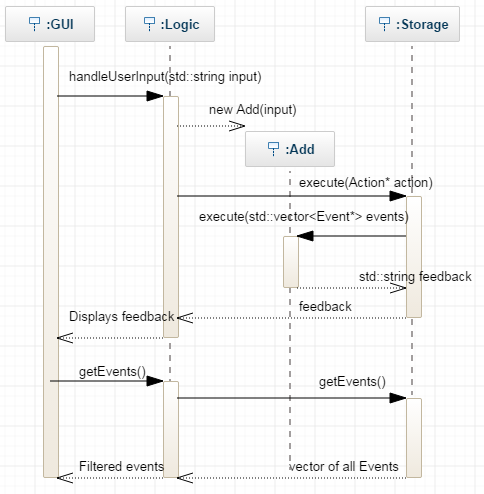
\includegraphics[width=\textwidth]{add_call_diagram}

The logic of the system is explained by the above sequence diagram.

\subsection{Key API}
The only call to the \texttt{Logic} component is made by the \texttt{GUI} when the \texttt{CommandLine::returnPressed()} signal is emitted. The function \texttt{Logic::handleUserInput(std::string)} will then proceed to process the input internally.

\subsection{Controller}

The controller is responsible for creating and executing commands. The user input is received by the controller and passed to the parser. The controller then receives the details of the user command from the parser and performs the action required (add, delete, edit, etc) detailed in the use cases in the appendix.

\begin{center}
\begin{tabular}{|l|r|}
Method                & Return Type \\
create(string input)  & pointer     \\
execute(string input) & pointer    
\end{tabular}
\end{center}

\subsection{Parser}

The parser deciphers user input and creates the relevant command based on the user input. It these sends the command to the controller for execution.

\begin{center}
\begin{tabular}{|l|r|}
Method              & Return Type \\
parse(string input) & pointer    
\end{tabular}
\end{center}

\subparagraph{1} All handlers(add, delete, etc) must use the parse() method and the argument must accept the string parameter.

\subparagraph{2} The parser should not modify the storage. If a task is supposed to be added, the parser should only generate the necessary fields of the task.

\subparagraph{3} All arguments which have an index, the parser must obtain the relevant information of the task which is then returned to the handlers.

\subparagraph{4} The exceptions thrown by the parser should be caught by the associated handler methods.

\subsection{Commands}
BoxIn currently recognizes the following user commands

\subparagraph{Sort}
Within the Command class, the information will be sorted out so it would be easier to parse out later.

\begin{center}
\begin{tabular}{  lrrl}
\hline
Add & Edit & Delete & Undo \\
\hline
Sort & Search & Display\\
\hline     
\end{tabular}
\end{center}

\newpage

\section{Storage}
The Storage class has only one purpose: to write all data stored in the Tasklist class into a file, and to retrieve the data in the file for BoxIn to use in the next session. Because the Storage class does not depend on other classes, it has low coupling which makes the software more efficient.
\subsection{Event}	 					
The Event class stores data created by the user. All of the data created by the user will be included here.
\subparagraph{set-parts}
The different set functions are vectors that stores the different sections of the user's data. \texttt{setName} for example, sets the name of the event to be inside a name folder. This allows the parser to use the data later on in a more efficient way.
\subparagraph{setFinish}
The \texttt{setFinish} function of the Event class saves the data completely when the user puts in all the parameter that is needed. It uses a vector as the structure to store all the information the user needs. 
\subsection{EventList}
The EventList implements a list based on the content the user inputs as data. It also returns the functions such as returning the data as vectors and sorting the data.
\subparagraph{eventList::contains(Events event)}
This method under event list returns a boolean of true or false and it works with logic to provide feedback if the event class is stored inside storage or not. If the event is already in the list, it can be use to edit later on.
\subparagraph{eventCompare}
The function of eventCompare allows the event storage class to determine which data goes to which category, it allows the data to sort based on date, location, time to store the data in a specific order.
\subsection{ActionStack}
The ActionStack Class saves the different events into files as well as returns the data when it is needed to be edited.
\subparagraph{undo}
When the user wants to undo a mistake that they have, they can undo using the undo method. This allows the stack to be popped off and be erased from the storage data. The stack will be popped off.


\begin{center}
\begin{tabular}{|l|r|}
Return Type                     & Method                                         \\
Vector<Event>                   & add(stringName)                                \\
Bool                            & delete(vector<Event> event)
\end{tabular}
\end{center}

\section{Appendix A}
\subsection{Full class diagram}
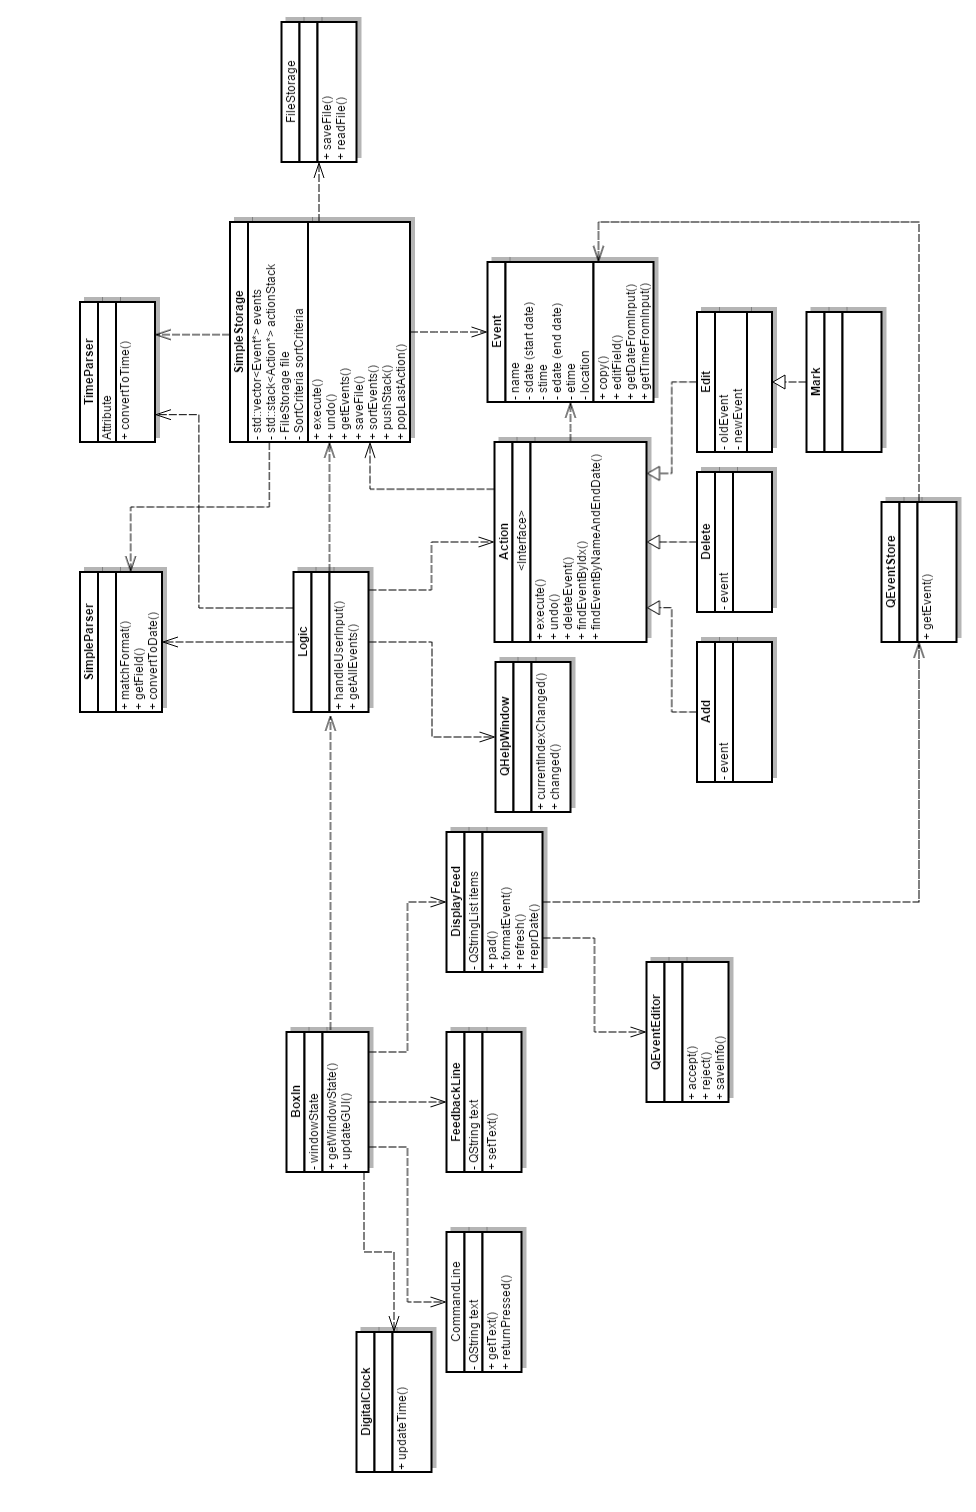
\includegraphics[width=\textwidth]{class_diagram}
\subsection{Use cases}
\begin{table}[ht]
\begin{tabular}{l|l}
Name                  & UC01:Add a new task                                                                                                                                                                                                                \\
Description           & To add a new task                                                                                                                                                                                                                  \\
Precondition          & BoxIn is currently running                                                                                                                                                                                                         \\
Basic course of event & \begin{tabular}[c]{@{}l@{}}1. User indicates the event that they want to add (Name, Date, Time, Place)\\and it has to be in this specific order\\ 2. BoxIn will give feedback indicating that the event has been added\end{tabular} \\
Alternative path      & \begin{tabular}[c]{@{}l@{}}1. One of the parameter is missing :\\ \\      1a. BoxIn responds that a parameter is missing and ask the user to try again\end{tabular}                                                                \\
Post Condition        & A new event is added and saved.                                                                                                                                                                                                   
\end{tabular}
\end{table}

\begin{table}[h]
\begin{tabular}{l|l}

Name                  & UC02: Delete a task                                                                                                                        \\
Description           & To delete an existing task.                                                                                                                                        \\
Pre Condition         & BoxIn is already running.                                                                                                                                          \\
Basic Course of Event & \begin{tabular}[c]{@{}l@{}}1. User types the command to delete an already existing task.\\ 2. The program deletes the task as per the user's command.\end{tabular} \\
Alternative Path      & \begin{tabular}[c]{@{}l@{}}1. If the task does not exist, the program displays the relevant message.\\ 2. Prompts the user to re-enter the command.\end{tabular}   \\
Post Condition        & The task is updated                                                                                                                                               
\end{tabular}
\end{table}

\begin{table}[h]
\begin{tabular}{l|l}

Name                  & Edit a task                                                                                                                                                                     \\
Description           & To edit an existing task                                                                                                                                                                                      \\
Pre Condition         & BoxIn is already running                                                                                                                                                                                      \\
Basic Course of Event & \begin{tabular}[c]{@{}l@{}}1. User types the command to edit an already existing task and \\specifying the relevant fields to be changed\\ 2. The program edits the task as per the user's command\end{tabular} \\
Alternative Path      & \begin{tabular}[c]{@{}l@{}}1. If the task does not exist, the program displays the relevant message.\\ 2. Prompts the user to re-enter the command.\end{tabular}                                              \\
Post Condition        & The task is updated                                                                                                                                                                                          
\end{tabular}
\end{table}

\begin{table}[h]
\begin{tabular}{l|l}
Name                  & UC04: Undo action                                                                                                                                   \\
Description           & To undo the previous command                                                                                                                                                \\
Pre Condition         & BoxIn is already running.                                                                                                                                                   \\
Basic Course of Event & 1. User types the command to undo the previous command.                                                                                                                     \\
Alternative Path      & \begin{tabular}[c]{@{}l@{}}1. If the previous action does not exist, the program displays the relevant \\message.\\ 2. Prompts the user to re-enter the command.\end{tabular} \\
Post Condition        & The task is deleted.                                                                                                                                                       
\end{tabular}
\end{table}

\begin{table}[h]
\begin{tabular}{l|l}

Name                  & UC05: Search task                                                                                                                                          \\
Description           & To search a task                                                                                                                                                                   \\
Pre Condition         & BoxIn is already running.                                                                                                                                                          \\
Basic Course of Event & \begin{tabular}[c]{@{}l@{}}1. User types the command to search for a task.\\ 2. The result is displayed.\end{tabular}                                                              \\
Alternative Path      & \begin{tabular}[c]{@{}l@{}}1. If the syntax does not match, prompts the user to re-enter the command.\\ 2. If the task does not exist, relevant message is displayed.\end{tabular} \\
Post Condition        & The task is undone.                                                                                                                                                               
\end{tabular}
\end{table}

\begin{table}[h]
\begin{tabular}{l|l}
Name                  & UC06: Sort task                                                                                                  \\
Description           & To sort tasks                                                                                                                            \\
Pre Condition         & BoxIn is already running.                                                                                                                \\
Basic Course of Event & \begin{tabular}[c]{@{}l@{}}1. User types the command to sort the tasks.\\ 2. The program displays the task in sorted order.\end{tabular} \\
Alternative Path        & 1. Sort criteria is not specified and tasks are sorted using the default order.             	                                                                                                                       \\
Post Condition        & -                                                                                                                                       
\end{tabular}
\end{table}

\begin{table}[h]
\begin{tabular}{l|l}

Name                  & UC07: Display task                                                                                      \\
Description           & To display a task                                                                                                               \\
Pre Condition         & BoxIn is already running.                                                                                                       \\
Basic Course of Event & \begin{tabular}[c]{@{}l@{}}1. User types the command to display the task.\\ 2. The program displays the task.\end{tabular}      \\
Alternative Path      & \begin{tabular}[c]{@{}l@{}}1. The relevant task does not exist.\\ 2. Program prompts the user to re-enter command.\end{tabular} \\
Post Condition        & -                                                                                                                              
\end{tabular}
\end{table}

\section{Appendix B:setting up}
To set up, you will need Windows Operating System, VS2012, Boost, and Git.
\subsection{1.QT}
The Visual Studio plugin for qt. You can find it at http://qt-project.org/downloads. 
Scroll to the bottom of the page and look for qt-vs-addin-1.2.3-opensource.exe. 
Then open Visual Studio. The top bar should show QT5 -> QT Options. Make 
sure that the correct version of QT is selected. 
\subsection{2.Boost}
boost - version 1.56, vc2012 (vc11.0), 32 bit. You can find it at 
http://sourceforge.net/projects/boost/files/boost-binaries/1.56.0/boost_1_56_0-
msvc-11.0-32.exe. Install to /local/boost_1_56_0 (the default folder). 
\subsection{3.Visual Studio plugin}
The Visual Studio plugin for qt. You can find it at http://qt-project.org/downloads. 
Scroll to the bottom of the page and look for qt-vs-addin-1.2.3-opensource.exe. 
Then open Visual Studio. The top bar should show QT5 -> QT Options. Make 
sure that the correct version of QT is selected. 
\subsection{4.Git}
You can download git from Github.com and register as a member, then clone the software and open the file and it should work out!

\end{document}